\documentclass[a4paper,11pt]{article}
\usepackage[utf8]{inputenc}
\usepackage{algorithmic}
\usepackage{algorithm}
\usepackage{pst-plot}
\usepackage{graphicx}
\usepackage{endnotes}
\usepackage{graphics}
\usepackage{floatflt}
\usepackage{wrapfig}
\usepackage{amsfonts}
\usepackage{amsmath}
\usepackage{verbatim}
\usepackage{hyperref}
\usepackage{multirow}
\usepackage{pdflscape}
 \usepackage{enumitem}

\usepackage{hyperref}
\hypersetup{pdfborder={0 0 0 0}}

\pdfpagewidth 210mm
\pdfpageheight 297mm 
\setlength\topmargin{0mm}
\setlength\headheight{0mm}
\setlength\headsep{0mm}
\setlength\textheight{250mm}	
\setlength\textwidth{159.2mm}
\setlength\oddsidemargin{0mm}
\setlength\evensidemargin{0mm}
\setlength\parindent{7mm}
\setlength\parskip{0mm}

\newenvironment{exercise}[3]{\paragraph{Exercise #1: #2 (#3pt)}\ \\}{
\medskip}
\newcommand{\question}[2]{\setlength\parindent{0mm}\ \\$\mathbf{Q_#1:}$ #2\ \\}

\author{\large{Ilya Kuzovkin, Raul Vicente}}
\title{\huge{Introduction to Computational Neuroscience}\\\LARGE{Practice on Single Neuron Models}}

\begin{document}
\maketitle

\textbf{A request:} Please track how long it will take to complete this set of exercises. Add this time to your final report.
\ \\

%
% Intro
%
In this session we will have a brief look on three different computational models of a neuron: McCulloch-Pitts, Intergrate-and-Fire and Hodgkin-Huxley.

%
% Logic gates
%
\begin{exercise}{1}{Logic gates}{1}
On the lecture we have seen how to construct \texttt{AND}, \texttt{OR} and \texttt{NOT} logic gates using the the McCulloch-Pitts model of a neuron. Your task is to construct more. Please construct the following two gates:
\begin{enumerate}
\itemsep 0em
	\item \texttt{NAND}
	\item \texttt{XOR}
\end{enumerate}
\paragraph{Hint 1}For the \texttt{XOR} gate you will need more than one neuron.
\paragraph{Hint 2}Same input can go simultaneously to several neurons.
\end{exercise}

%
% Integrate and Fire
%
\begin{exercise}{2}{Integrate and Fire neuron model}{2.5}
Integrate and Fire neuron accumulates voltage until it reaches the \emph{threshold}. After that it fires and resets voltage back to initial value. In this exercise we will model behaviour of such neuron and study its properties. Follow the instructions in the \texttt{integratefire.m} file and report all figures, essential pieces of code, answers, interpretations and conclusions you will make during the work.

\paragraph{Note} The \texttt{TODO} marker will indicate the places where you have to do something: complete the code, plot and report a figure, give an interpretation, etc.\\
\ \\
The very final result in this exercise should look something like this
\begin{figure}[H]
   \centering
   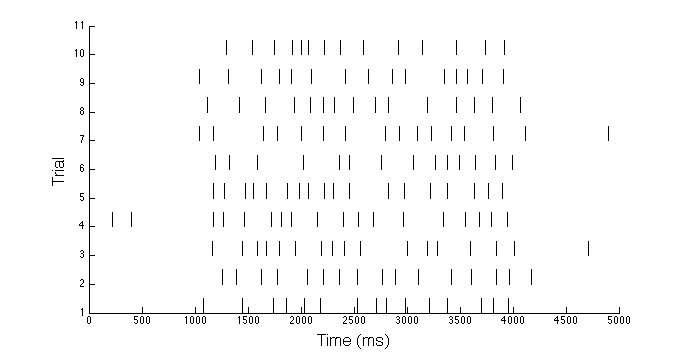
\includegraphics[width=0.8\textwidth]{raster_plot.png} 
   \caption{10 trials of data generated using Integrate-and-Fire neuron model.}
   \label{fig:rasterplot}
\end{figure}
\end{exercise}


%
% Hodgkin-Huxley
%
\begin{exercise}{3}{Hodgkin-Huxley neuron model}{1.5}
Hodgkin-Huxley model is considered to be the most important computational neuronal model in the neuroscience today. We have the model already implemented in the file \texttt{HH0.m}, study it. Follow the instructions in the \texttt{hodgkinhuxley.m} file and report all figures, thoughts, interpretations and conclusions you will have during the work.

\paragraph{Note} The \texttt{TODO} marker will indicate places where you have to do something: complete the code, plot and report a figure, give an interpretation, etc.
\end{exercise}


%
% Integrate and Fire with synapses
%
\begin{exercise}{4}{Integrate and fire with synapses}{1}
In this exercise we will play with somewhat more realistic version of integrate-and-fire model, which receives input not from constant current as we did before, but from incoming (\emph{presynaptic}) spikes. \emph{Temporal summation} can lead to the voltage reaching the threshold and then the \emph{postsynaptic} neuronal response (firing) occurs. Read the tutorial\footnote{\url{http://www.dreamincode.net/forums/topic/72868-a-simple-neuron-model-the-integrate-and-fire-neuron}} and study the code given there. Slightly modified code is provided to you in the file \texttt{integratefiresynapses.m}. Your task is to compe up with three different configurations of spikes on the line 41:
\begin{enumerate}
	\item Inside the time window from 0 to 200 ms there will be 4 incoming spikes and 1 output spike.
	\item Inside the time window from 200 to 400 ms there will 5 incoming spikes and 0 output spikes.
	\item Is is possible to produce 2 output spikes with 5 incoming spikes? If yes, then produce it in time window 400 to 600 ms, if not show the maximal voltages you can achieve with 5 input spikes.
\end{enumerate}
\end{exercise}


%
% SR latch
%
\begin{exercise}{X*}{Simulate memory with $\neg S$-$\neg R$ latch}{bonus 2}
In electronics there is a circuit, which can \emph{store} a state. This means that after we \emph{set} it to some state, it will remain there until we \emph{reset} it. The whole thing is called \emph{D latch}, it has a sub-part called \emph{SR latch}, which again has a subpart called \emph{$\neg S$-$\neg R$ latch}.
\begin{enumerate}
\itemsep 0em
	\item Watch this video \url{https://www.youtube.com/watch?v=PCT76PsDr6g} (until 12:26)
	\item and build $\neg S$-$\neg R$ latch using McCulloch-Pitts neurons. 
\end{enumerate}
\end{exercise}


\ \\
\ \\
\ \\
\ \\
\ \\
Please submit a \texttt{pdf} report with answers to the questions and comments about your solutions. Include figures, explanations and essential pieces of code. Do not include the code itself as a separate file, your report should give good understanding of what you have done. Please mark how long it took to complete this set of exercises. Upload the \texttt{pdf} to the practice session page on the course website.

\end{document}










